\documentclass{report}
\usepackage[T1]{fontenc}
\usepackage{babel}
\usepackage[dvipsnames,table]{xcolor}
\usepackage{ulem}
%https://mirrors.dotsrc.org/ctan/macros/luatex/latex/emoji/emoji-doc.pdf
%\usepackage{emoji}
\usepackage[framemethod=tikz]{mdframed}
%\usepackage{marginnote}
%\setlength{\marginparwidth}{3cm}
%\setlength{\marginparsep}{1cm}
\usepackage{amsmath,amsfonts,amssymb,amsthm}
\usepackage{booktabs}
\usepackage{multirow}
%\usepackage{lilyglyphs} %https://www.ctan.org/pkg/lilyglyphs
\usepackage{array}
\usepackage{boldline}
\usepackage{etoolbox}
\usepackage[labelformat=empty]{caption}
%\usepackage{wasysym}
%\usepackage{fancyhdr}
\usepackage{tabularx}
\usepackage{csquotes}
%\usepackage{animate}
%\usepackage{hyperref}
\usepackage{tikz}
\usepackage{pgfplots}
\usepackage{tikzfill}
\usetikzlibrary{intersections, pgfplots.fillbetween, fill.image}
\pgfdeclarelayer{back}
\pgfsetlayers{back,main}
%\usepackage{arsclassica}


%\titleformat{\chapter}[block]%
        {\normalfont\Large\sffamily}%
        {{\color{halfgray}\chapterNumber\thechapter%
        \hspace{10pt}\vline}  }{10pt}%
        {\spacedallcaps}[\chapterdecoration]

\definecolor{halfgray}{gray}{0.55}

\newcommand\chapterdecoration{%
\begin{tikzpicture}[remember picture,overlay,shorten >= -10pt]

\coordinate (aux1) at ([yshift=-15pt]current page.north east);
\coordinate (aux2) at ([yshift=-410pt]current page.north east);
\coordinate (aux3) at ([xshift=-4.5cm]current page.north east);
\coordinate (aux4) at ([yshift=-150pt]current page.north east);

\begin{scope}[halfgray!40,line width=12pt,rounded corners=12pt]
\draw
  (aux1) -- coordinate (a)
  ++(225:5) --
  ++(-45:5.1) coordinate (b);
\draw[shorten <= -10pt]
  (aux3) --
  (a) --
  (aux1);
\draw[opacity=0.6,halfgray,shorten <= -10pt]
  (b) --
  ++(225:2.2) --
  ++(-45:2.2);
\end{scope}
\draw[halfgray,line width=8pt,rounded corners=8pt,shorten <= -10pt]
  (aux4) --
  ++(225:0.8) --
  ++(-45:0.8);
\begin{scope}[halfgray!70,line width=6pt,rounded corners=8pt]
\draw[shorten <= -10pt]
  (aux2) --
  ++(225:3) coordinate[pos=0.45] (c) --
  ++(-45:3.1);
\draw
  (aux2) --
  (c) --
  ++(135:2.5) --
  ++(45:2.5) --
  ++(-45:2.5) coordinate[pos=0.3] (d);   
\draw 
  (d) -- +(45:1);
\end{scope}
\end{tikzpicture}%
}



\theoremstyle{definition}
\newtheorem*{definition}{Definition}%[section]



\newcommand\chapterdecoration[1]{%
%\begin{tikzpicture}[remember picture,overlay,shorten >= -10pt]
\begin{tikzpicture}[remember picture,overlay]
\coordinate (dectopright) at ([yshift=-100] current page.north east);
\coordinate (dectophelp) at ([xshift=-150] dectopright);
\coordinate (dectopleft) at ([yshift=-75] dectophelp);
\coordinate (decbottomright) at ([yshift=-500] dectopright);
\coordinate (decbottomhelp) at ([yshift=-500] dectophelp);
\coordinate (decbottomleft) at ([yshift=75] decbottomhelp);


\foreach \x in {10,20,...,150} 
  {
   \path[draw, fill=white]  
    ([yshift=- \x] dectopright)
   --  ([xshift= \x , yshift= -\x] dectopleft) 
   -- ([xshift=  \x , yshift= \x] decbottomleft) 
   -- ([yshift=\x] decbottomright) 
   -- ([yshift=\x + 4.5] decbottomright) 
   -- ([xshift= \x +4.5 , yshift= \x +5] decbottomleft) 
   -- ([xshift= \x  +4.5, yshift=- \x - 5] dectopleft) 
   -- ([yshift= - \x -5] dectopright)
   -- ([yshift=- \x] dectopright);
 

  }

\begin{pgfonlayer}{back}
\path[draw, fill stretch image=#1, fill image opacity=0.2] %, fill image scale=0.5
    (dectopright) -- (dectopleft) -- (decbottomleft) -- (decbottomright) -- (dectopright);
\end{pgfonlayer}
\end{tikzpicture}
}


\newcommand{\chapterize}[4]{
  \newpage
  \chapterdecoration{#4}
  \vspace{80pt}
  \begin{center}
  \end{center}
  \begin{flushleft}
   \textbf{\Huge #1}
  \vspace{100pt}
  
  \parbox{9cm}{
    {\color{gray} #2}\\
    \hrule
    \vspace{20pt}
    #3
    
  }
  \end{flushleft}
  \newpage
}




\DeclareRobustCommand{\sovs}{
 \mbox{
  {\Large $\mathbb{S}_{O}$  }
  {\kern-1em\raise.8ex\hbox{V}\kern-.125em\@}
  {\kern-0.3em$\mathbb{S}$}
 }
}

\DeclareRobustCommand{\sectionsovs}{
 \mbox{
  {\Huge $\mathbb{S}_{O}$  }
  {\kern-1em\raise.8ex\hbox{V}\kern-.125em\@}
  {\kern-0.3em$\mathbb{S}$}
 }
}

\DeclareRobustCommand{\sectionsovsen}{
 \mbox{
  {\Huge $\mathbb{S}_{O}$  }
  {\kern-1em\raise.8ex\hbox{V}\kern-.125em\@}
  {\kern-0.3em$\mathbb{S}$}
  {\Huge $\sum_{}$ }
  {\kern-0.3em$\mathbb{N}$}
 }
}


\DeclareRobustCommand{\sovseneer}{
\mbox{
  {\Large $\mathbb{S}_{O}$  }
  {\kern-1em\raise.8ex\hbox{V}\kern-.125em\@}
  {\kern-0.3em$\mathbb{S}$}
  {\kern-0.3em\hbox{e}}
  {\kern-0.3em$\mathbb{N}$}
  {\Large $\sum_{}^{e}$ }
  {\kern-0.3em\hbox{R}}
 }
}

\DeclareRobustCommand{\sovsing}{
 \mbox{
  {\Large $\mathbb{S}_{O}$  }
  {\kern-1em\raise.8ex\hbox{V}\kern-.125em\@}
  {\kern-0.3em$\mathbb{S}_{\mathbb{I}ng}$}
 }
}

\mdfdefinestyle{scene}{
  leftmargin=-0.2cm,
  rightmargin=-2cm,
  roundcorner=10pt,
  frametitlerule=true,
  frametitlebackgroundcolor=gray!20
}


\mdtheorem[style=scene]{scene}{Scene}


%\kern-.36em%
%
 % {\sbox\z@ T%
%    \vbox to\ht\z@{\hbox{\check@mathfonts
 %   \fontsize\sf@size\z@  
%    \math@fontsfalse\selectfont
%    A}%
%  \vss}%
%}%
%\kern-.15em%
%\TeX}

\author{Sunetiago Hansen}
\title{Simrebogen}

\colorlet{cfemale}{RubineRed}
\colorlet{cmale}{BlueViolet}
\colorlet{cdanish}{Gray}
\definecolor{cfigsovs}{RGB}{18,37,103}
\definecolor{cfigsalsa}{RGB}{138,0,0}
\definecolor{cattack}{RGB}{185,0,185}

\newcommand{\scactorf}[1]{{\color{cfemale}\textbf{\textit{#1}}}}
\newcommand{\scactorm}[1]{{\color{cmale}\textbf{\textit{#1}}}}

\newcommand{\dude}{\scactorm{Dude }}
\newcommand{\dudetwo}{\scactorm{Dude$_{2}$}}
\newcommand{\gal}{\scactorf{Gal }}


\newcommand{\figsalsa}[1]{
  {\color{cfigsalsa}
    {\fontfamily{lmdh}\selectfont #1 }
  }
}

\newcommand{\figsovs}[1]{
  {\color{cfigsovs}
    {\fontfamily{lmdh}\selectfont #1 }
  }
}

\newcommand{\attack}[1]{
  {\color{cattack}
    {\fontfamily{qtm}\selectfont \textit{#1} }
  }
}

\newcommand{\attackdesc}[1]{
    {\fontfamily{qtm}\selectfont \textit{#1} }
}

\newcommand{\salsaguapea}{\figsalsa{guapea}}
\newcommand{\salsavuelta}{\figsalsa{vuelta}}
\newcommand{\salsavamos}{\figsalsa{vamos arriba}}
\newcommand{\salsadile}{\figsalsa{dile que no}}
\newcommand{\salsaenchufla}{\figsalsa{enchufla}}
\newcommand{\salsavacilala}{\figsalsa{vacílala}}
\newcommand{\salsauno}{\figsalsa{el uno}}
\newcommand{\salsados}{\figsalsa{el dos}}
\newcommand{\salsasetanta}{\figsalsa{setenta}}
\newcommand{\salsasetantayuno}{\figsalsa{setenta y uno}}
\newcommand{\salsasetantaydos}{\figsalsa{setenta y dos}}

\newcommand{\Salsaguapea}{\figsalsa{Guapea}}
\newcommand{\Salsavuelta}{\figsalsa{Vuelta}}
\newcommand{\Salsavamos}{\figsalsa{Vamos arriba}}
\newcommand{\Salsadile}{\figsalsa{Dile que no}}
\newcommand{\Salsaenchufla}{\figsalsa{Enchufla}}
\newcommand{\Salsavacilala}{\figsalsa{Vacílala}}
\newcommand{\Salsauno}{\figsalsa{El uno}}
\newcommand{\Salsados}{\figsalsa{El dos}}
\newcommand{\Salsasetanta}{\figsalsa{Setenta}}
\newcommand{\Salsasetantayuno}{\figsalsa{Setenta y uno}}
\newcommand{\Salsasetantaydos}{\figsalsa{Setenta y dos}}

\newcommand{\sovsguapea}{\figsovs{begynderen}}
\newcommand{\sovsvuelta}{\figsovs{rundtenom}}
\newcommand{\sovsvamos}{\figsovs{fremad Ama'r}}
\newcommand{\sovsdile}{\figsovs{grønlændervendingen}}
\newcommand{\sovsenchufla}{\figsovs{frem \& tilbage}}
\newcommand{\sovsvacilala}{\figsovs{snurretoppen}}
\newcommand{\sovsuno}{\figsovs{etteren}}
\newcommand{\sovsdos}{\figsovs{to'eren}}
\newcommand{\sovssetanta}{\figsovs{70'eren}}
\newcommand{\sovssetantayuno}{\figsovs{71'eren}}
\newcommand{\sovssetantaydos}{\figsovs{72'eren}}


\newcommand{\Sovsguapea}{\figsovs{Begynderen}}
\newcommand{\Sovsvuelta}{\figsovs{Rundtenom}}
\newcommand{\Sovsvamos}{\figsovs{Fremad Ama'r}}
\newcommand{\Sovsdile}{\figsovs{Grønlændervendingen}}
\newcommand{\Sovsenchufla}{\figsovs{Frem \& tilbage}}
\newcommand{\Sovsvacilala}{\figsovs{Snurretoppen}}
\newcommand{\Sovsuno}{\figsovs{Etteren}}
\newcommand{\Sovsdos}{\figsovs{To'eren}}
\newcommand{\Sovssetanta}{\figsovs{70'eren}}
\newcommand{\Sovssetantayuno}{\figsovs{71'eren}}
\newcommand{\Sovssetantaydos}{\figsovs{72'eren}}

\newcommand{\attknytter}{\attack{knytter}}
\newcommand{\attsvinger}{\attack{svinger}}
\newcommand{\attflemming}{\attack{Flemming}}
\newcommand{\attbagknytter}{\attack{bag-knytter}}
\newcommand{\attsideaxe}{\attack{væltet økse}}
\newcommand{\attlosser}{\attack{losser}}
\newcommand{\atttrykker}{\attack{trykker}}
\newcommand{\attsidetrykker}{\attack{væltet trykker}}
\newcommand{\atthestehilsen}{\attack{heste-hilsen}}
\newcommand{\attfootjuglar}{\attack{fod-jonglør}}
\newcommand{\attrambuk}{\attack{rambuk}}
\newcommand{\attsuperman}{\attack{Superman}}
\newcommand{\attkaffekage}{\attack{kaffe \& kage}}
\newcommand{\attkneeler}{\attack{knæler}}
\newcommand{\atttakedown}{\attack{ne'mæda}}

\newcommand{\Attknytter}{\attack{Knytter}}
\newcommand{\Attsvinger}{\attack{Svinger}}
\newcommand{\Attflemming}{\attack{Flemming}}
\newcommand{\Attbagknytter}{\attack{Bag-knytter}}
\newcommand{\Attsideaxe}{\attack{Væltet økse}}
\newcommand{\Attlosser}{\attack{Losser}}
\newcommand{\Atttrykker}{\attack{Trykker}}
\newcommand{\Attsidetrykker}{\attack{Væltet trykker}}
\newcommand{\Atthestehilsen}{\attack{Heste-hilsen}}
\newcommand{\Attfootjuglar}{\attack{Fod-jonglør}}
\newcommand{\Attrambuk}{\attack{Rambuk}}
\newcommand{\Attsuperman}{\attack{Superman}}
\newcommand{\Attkaffekage}{\attack{Kaffe \& kage}}
\newcommand{\Attkneeler}{\attack{Knæler}}
\newcommand{\Atttakedown}{\attack{Ne'mæda}}



\newcommand{\chapgap}{{\vspace{8pt}}}




\begin{document}




%----------------------------------------------------------------------------------------
%	TITLE PAGE
%----------------------------------------------------------------------------------------

\begin{titlepage} % Suppresses headers and footers on the title page

	\raggedleft % Right align everything
	
	\vspace*{\baselineskip} % Whitespace at the top of the page
	
	%------------------------------------------------
	%	Author
	%------------------------------------------------
	
	{\Large Sunetiago Hansen} % Author name
	
	\vspace*{0.167\textheight} % Whitespace before the title
	
	%------------------------------------------------
	%	Title and subtitle
	%------------------------------------------------
	
	%\textbf{\LARGE The Big Book of}\\[\baselineskip] % First title line
	
	{\textcolor{Gray}{\Huge Simrebogen v. 1.0}}\\[\baselineskip] % Main title line which draws the focus of the reader
	
	{\Large\textit{The \sovs manifesto}} % Subtitle
	
	\vfill % Whitespace between the titles and the publisher
	\begin{center}
           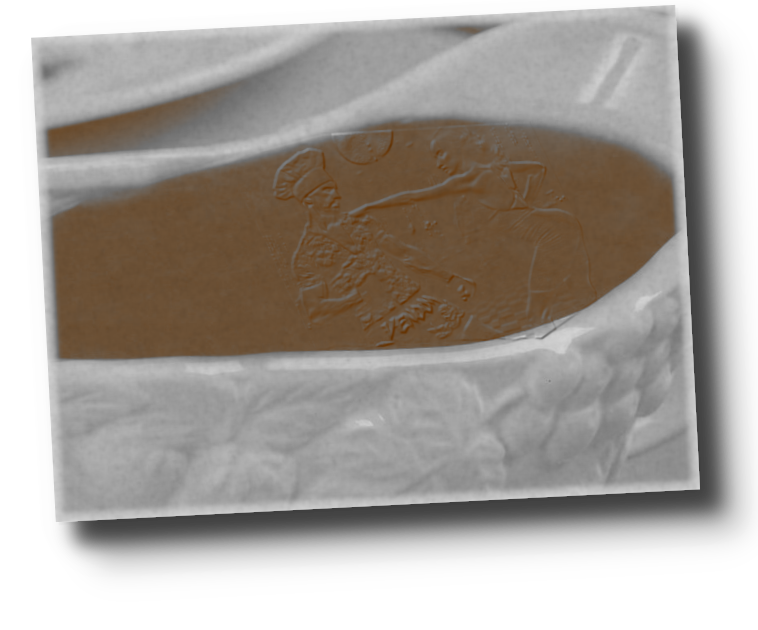
\includegraphics[scale=2.2]{Frontpage/sovs-front-page}
	\end{center}

	%------------------------------------------------
	%	Publisher
	%------------------------------------------------
	
	%{\large ~~\plogo} % Publisher and logo
	
	\vspace*{3\baselineskip} % Whitespace at the bottom of the page

\end{titlepage}



\chapterize{Smørbolle}
  {
     Bland tiloversbleven fedtstof fra tilberedning af rettens kød (f.eks. svinefedt der er dryppet fra flæskesteg eller stegefedtet fra stegte andelår) med smør i en gryde, og opvarm ved svag varme.\\ 

    \chapgap

     Tilsæt under omrøring mel indtil blandingen ikke længere er flydende. Spred smørbollen ud i gryden, og lad den stå ved lav varme indtil smørbollen udskiller en let nødde-agtig lugt. 
  }
  {
   Mix leftover fat from cooking the meat of the dish (eg lard that has dripped from roast pork or the fat from fried duck legs) with butter in a saucepan at low heat. \\

    \chapgap

   Add flour while stirring until the mixture is no longer runny. Spread the butter ball out in the pan and leave it on low heat until the butter ball emits a slightly nutty smell.
  
  }{01-Intro/chapter-deco}
  
\section*{Why do we need another fusion dance style?}
... Not to mention another martial art? \textit{Surely, any civilized major city in the Western World has a very diversified offering of both dance- and martial arts-classes, so can't we just sign up for one of those?}\\
Sure you can, and I strongly urge you to sign up for one or several of both and find a couple that you like. But that shouldn't stop you from \sovsing. Hopefully, those classes will only increase your \textit{rizz} and your skillset as a \sovseneer

\paragraph{}
\sovs is not another elaborated curriculum of neither dancing nor fighting, and there is no need to set up a Duolingo rutine to learn Spanish, Chinese or Japanese in order to \sovs\\
The fundamental principles of \sovs can - and more than likely \textit{will} - be applied to any style of dancing, but \sovs specifically refers to the fusion of \textbf{\textit{Cuban Salsa}} with the martial arts.\\
Whereas the type of \textit{dancing} to use as framework for the expressions of \sovs is fixed to Cuban Salsa, the choice of \textit{martial art} applied by the \sovseneer is completely free.

\section*{\sovs optimizes the mating ritual}
For as long as anyone can remember, the dancefloor has been the goto place for humans to perform initial steps of the mating ritual\footnote{During the last 10+ years, online dating has seen an incredible rise in popularity, but seeing as the author of this book has no experience what-so-ever in the world of online dating, we will base the discussion on data pre-dating the age of online dating. I'm sure it's just a fad anyways}, with very little change to the overall principles of interaction. Consider the following scene.

\begin{scene*}[In the club]
\dude is in the club looking for a compatible mate, when he locks eyes with \scactorf{Gal}, who is in the club with exactly the same intentions. Now, \scactorf{Gal} wants to make sure that the communication with a potential mate will work before indulging in a night of passion. She takes to the dance floor hoping to get a sense of \dude's physical expressiveness. \dude would like to engage in a night of passion with \scactorf{Gal}, but doesn't know the first thing about dancing. Being afraid that he will make a fool of himself on the dance-floor, he boosts the ol' self-confidence with a bottle of $37.5\%$ courage-potion from the bar and a couple of lines of concentrated coca leaves extract in the bathroom, before going to the dance floor and making a complete fool of himself.\\
Hellbent on proving his peak physical state to \scactorf{Gal}, he picks a fight with \dudetwo. \scactorf{Gal} get's upset by the foolish display, \dudetwo get's a couple of black eyes and a trip to the dentist. \dude doesn't get any.
\end{scene*}

\newpage

{\color{cfemale}{\subsection*{Benefits of \sovs for \textit{her}}}}

\subsubsection*{\sovs provides a clear and easy way to show disinterest}
Not interested in the person you are dancing with? Easy: \attknytter to the face. Is he having a hard time getting the message? \atttrykker to the chest, and off you go. Simple as that.

\subsubsection*{\sovs is built to test physical fitness}
Maybe interested in the person that you are dancing with, but want to ensure that he has the proper lower body endurance to keep up with you? Easy: go for a couple of \attlosser$\!$s to the thighs. If he is still standing before your shins tire from the testing, he'll probably do fine later on.

\subsubsection*{\sovs is perfect for showing interest}
Think your dancing partner is hot shit, and want to unambiguosly tell him that it's about time for the two of you to leave this place and head to more appropriate lodgings? Go for the take-down. That's a language that even the drunkest drunkard will understand. 


\newpage
{\color{cmale}{\subsection*{Benefits of \sovs for \textit{him}}}}

\subsubsection*{It is a lot more fun being punched by women than other dudes}
\begin{scene*}[In the dojo/mouh goon/gym]
\scactorm{Instructor}: \textit{Watch closely as I demonstrate this cool technique. [does cool technique]\\
Now you do! And focus on technique instead of beating each other into a pulp!}\\
\dude and \dudetwo: \textit{YES SENSEI/SIFU/SIR!}\\
\paragraph{}
$\cdots$ \textit{2 minutes later} $\cdots$\\
\paragraph{}
\dude and \dudetwo: \textit{[beating each other into a pulp]}\\
\scactorm{Instructor}: you are not practicing the technique!
\dude: \textit{Well, we \textbf{were} practicing the technique, but then \dudetwo punched me in the gut, and you know how there is something about \dudetwo that makes you just want to punch him in the face and well...}\\

\scactorm{Instructor}:
\begin{center}
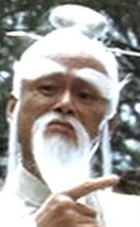
\includegraphics[scale=0.5]{01-Intro/concerned-sifu}
\end{center}
\end{scene*}

I'm sure that anyone who has put more than 5 hours into the martial arts will reckognize the scenario above, and let's face it: it's a lot more fun to practice techniques with women than men. Unfortunately, in most places where martial arts is practiced, the woman:man ratio doesn't really favor this fact.\\
\sovs greatly remedies this by taking technique-practice onto the dance floor! 

\newpage
\subsubsection*{\sovs increases the vocabulary of movements on the dance floor}
Have you ever taken dance lessons? If so, you might have come across an instructor who has uttered such words as: \textit{...and then the man shows off his \textbf{machismo} by doing this movement [proceeds to perform movement that conveys very \textbf{little} machismo]}\\
How the hell are you supposed to express your \textit{inner caveman}, if you are only allowed to use a \textit{girlish} vocabulary? I bet you don't feel girlish when you are \textit{ducking/slipping} punches or taking \textit{shin-kicks} to the thighs during sparring, right?\\ 
Well, there you go!

\subsubsection*{\sovs let's you see another side of her before comitting to any type of \textit{tomfoolery}}
You can tell a lot about a woman by how she punches you in the face, but unless you have a really annoying personality you are not likely to see that side of her until you are knee-deep in dirty diapers, and by then it's sorta too late. To this end, \sovs is the perfect \textit{try before you buy}!




\chapterize{Opbagning af \sectionsovsen}
  {
   Når smørbollen begynder at afgive en let nøddeagtig duft, tilsættes ca. 2 dl. mælk eller fløde, og blandingen bringes til kogning. Det er på dette tidspunkt anbefalelsesværdigt at skrue op for varmen på blusset, men det er vigtigt at dette sker under konstant omrøring, da en sovs der er brændt på er en dårlig sovs.\\

    \chapgap

   Når blandingen er bragt til kogning, tilsættes en yderligere mængde mælk og blandingen bringes igen til kogning. Denne process fortsættes indtil den ønskede mætning og mængde sovs er tilvejebragt.
  }
  {
   When the butter bun starts to give off a slightly nutty scent, add approx. 2 dl. milk or cream and bring the mixture to boil. At this point it is advisable to turn up the heat on the burner, but it is important that this is done with constant stirring, as a sauce that is burnt is a bad sauce.\\

    \chapgap

    When the mixture is brought to a boil, a further amount of milk is added and the mixture is again brought to boil. This process is repeated until the desired saturation and amount of sauce is achieved.
  }{02-Description/chapter-deco}

\chapter*{How to \sectionsovs}

Any lunatic can do some martial arts classes, go for a couple of rounds of Cuban Salsa and come up with the idea to combine the two (the mere existence of this manifest sort of proves this point), but the secret sauce (pun intended) is in describing \textit{how} to combine the two, which is exactly what will be done in this chapter. \\
The purpose is not to do a complete enumeration of all possible combinations of Cuban Salsa figures with attacks and defences from all sub-categories of martial arts, but to demonstrate \textit{some} ways in which to combine the two, that will allow the reader to get started with experimenting on the dance floor and take part in the cancerous/viral growth of the \sovs underworld.\\
If you are totally new to either Cuban Salsa or the martial arts, you may very well benefit from pausing the consumption of this manifest, do an internet search for ``Cuban Salsa intro course'' or ``basic punching'' respectively and invest a total of 15 minutes in whatever online videos will undoubtedly be presented in abbundance. The popular online video services have brief demonstrations of all salsa figures listed here, and a 40 second demonstration will probably do more for the overall understanding of a figure, than what my limited skills in terms of drawing and providing textual descriptions can. \\

\subsection*{Rules \& ground principles of \sovs}
On the dance floor, \sovs imposes the following few and easy-to-remember rules and restrictions:

\begin{enumerate}
  \item as in Cuban Salsa, the \dude is responsible for \textit{leading}
  \item only the \gal is allowed to attack
  \item any attack and defence is allowed, as long as it does not obstruct the continuation of the dance
\end{enumerate}

The rule oulined in 3), is formalized by the \text{The Flow Must Go On}-definition:

\begin{definition}[The Flow Must Go On]
\gal is allowed to attack \dude in any and all ways thinkable, that would not prevent the succesful execution of a \textit{Rueda de Casino} given proper defence by \dude
\end{definition}

Another way of saying this is: \textit{``do what you must, but make sure to be done by the end of the figure''}. Yet another way to say the same thing is: \textit{``you may kill your partner, but don't kill the \textbf{rhythm}!''}.\\
In the descriptions that follow, parts of the currently established \sovs glossary is used. The complete \sovs nomenclature as of the current time of writing, is presented in the following chapter. 

\pagebreak{}
\section*{Examples of figures}
\subsection*{\Sovsguapea [\Salsaguapea]}
\begin{center}
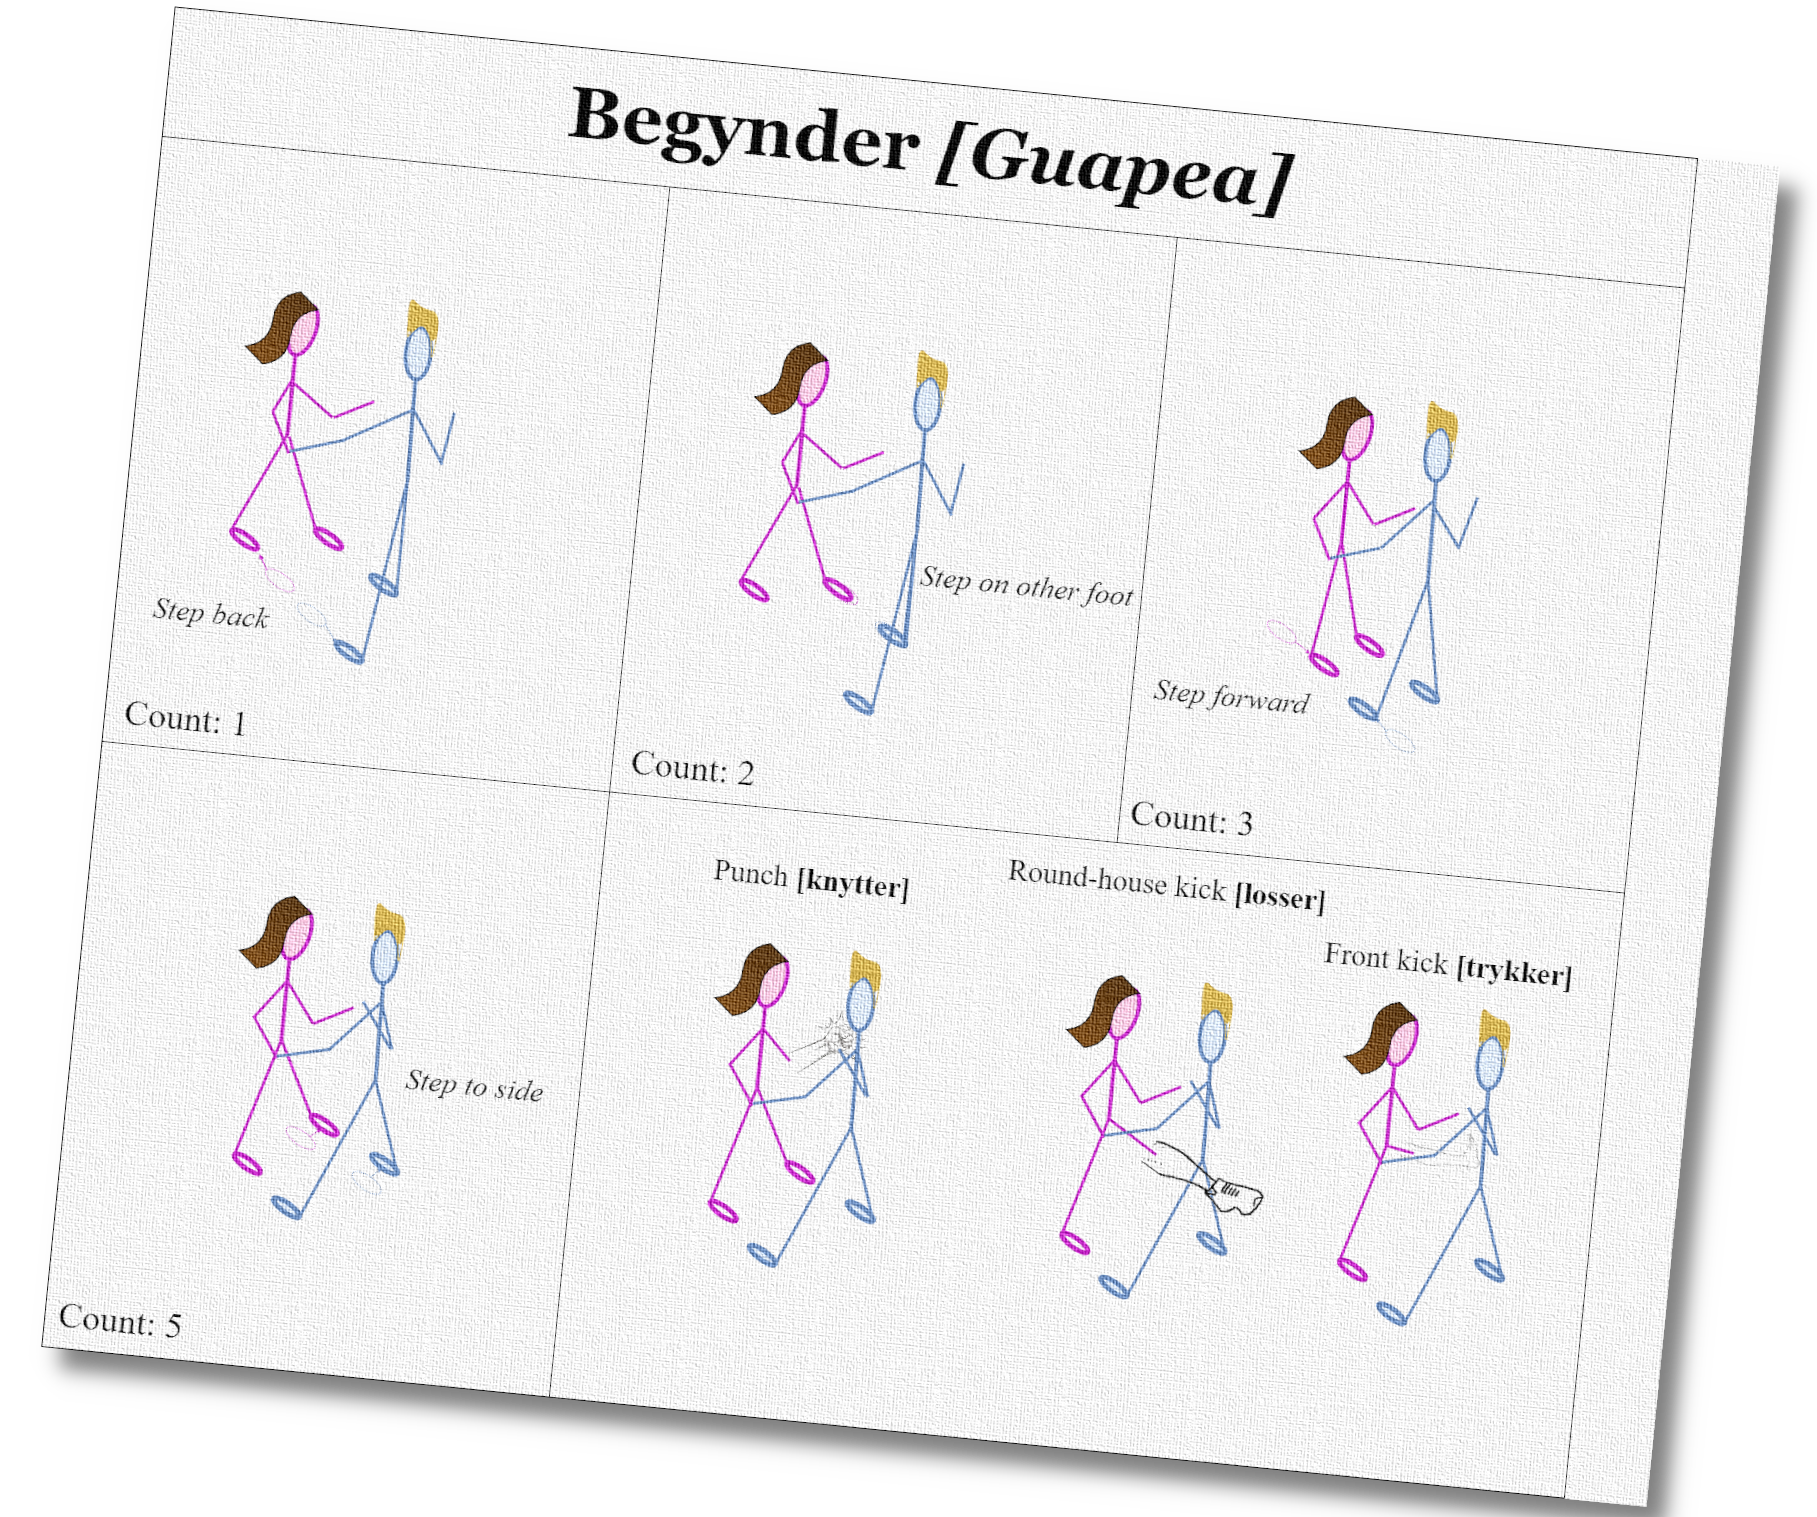
\includegraphics[scale=0.15]{02-Description/diagram-guapea-present}
\end{center}


\subparagraph*{Description}
If you, filled to the brim with anticipation of becoming the next Latin Dance God take your first Cuban Salsa intro class, it is very likely that you will first be shown a few basic steps, and when it comes time to partner up, the \salsaguapea is the first series of steps that you are taught. In \sovs, we call this same move \sovsguapea. And why is that you ask? Because it is so darn \textit{easy}!\\
\Sovsguapea starts off in the open position, with the 2 facing each other and \dude holding \scactorf{Gal's} \textbf{right} hand in his own \textbf{left} hand. On the first count both of them step back on the foot closest to the hand used for holding hands (i.e. \dude steps back on his left foot and \gal steps back on her right foot). On the second count, both step in place with the opposite foot and on the third count they both bring their hind foot forward to it's starting position. In salsa, counts 4 and 8 are generally upheld like the Abrahamic religions uphold their day of rest, and as such, are spent on quiet contemplation. On count 5, both parties step outwards with the foot closest to their \textit{free} hand as their free hands meet in the middle, palms facing towards each other. On count 6, both step in place with their opposite foot, and on count 7 they return to the starting position. 
\subparagraph*{Suggestions for attacking}
The most obvious times for \gal to attack is when she is already engaged in forward movement, either as she steps forward on count 3, or as she brings her hand towards \dude on count 5.\\
Seeing as the distance between the 2 is rather narrow, it can be hard for her to land a \atttrykker (forward-pushing kick), but the distance is quite suitable for a \attlosser (round-house kick) and pretty much any type of punch should be well within reach of it's target. If \gal is feeling frisky, she might even go for a little combination punching and try to hit \dude with for instance a quick \textit{jab-hook combo} or a \attflemming (faking a punch to the head, and diving for a weaselly gut-punch). Really, the sky is the limit!  


\pagebreak{}
\section*{\Sovsdile [\Salsadile]}
\begin{center}
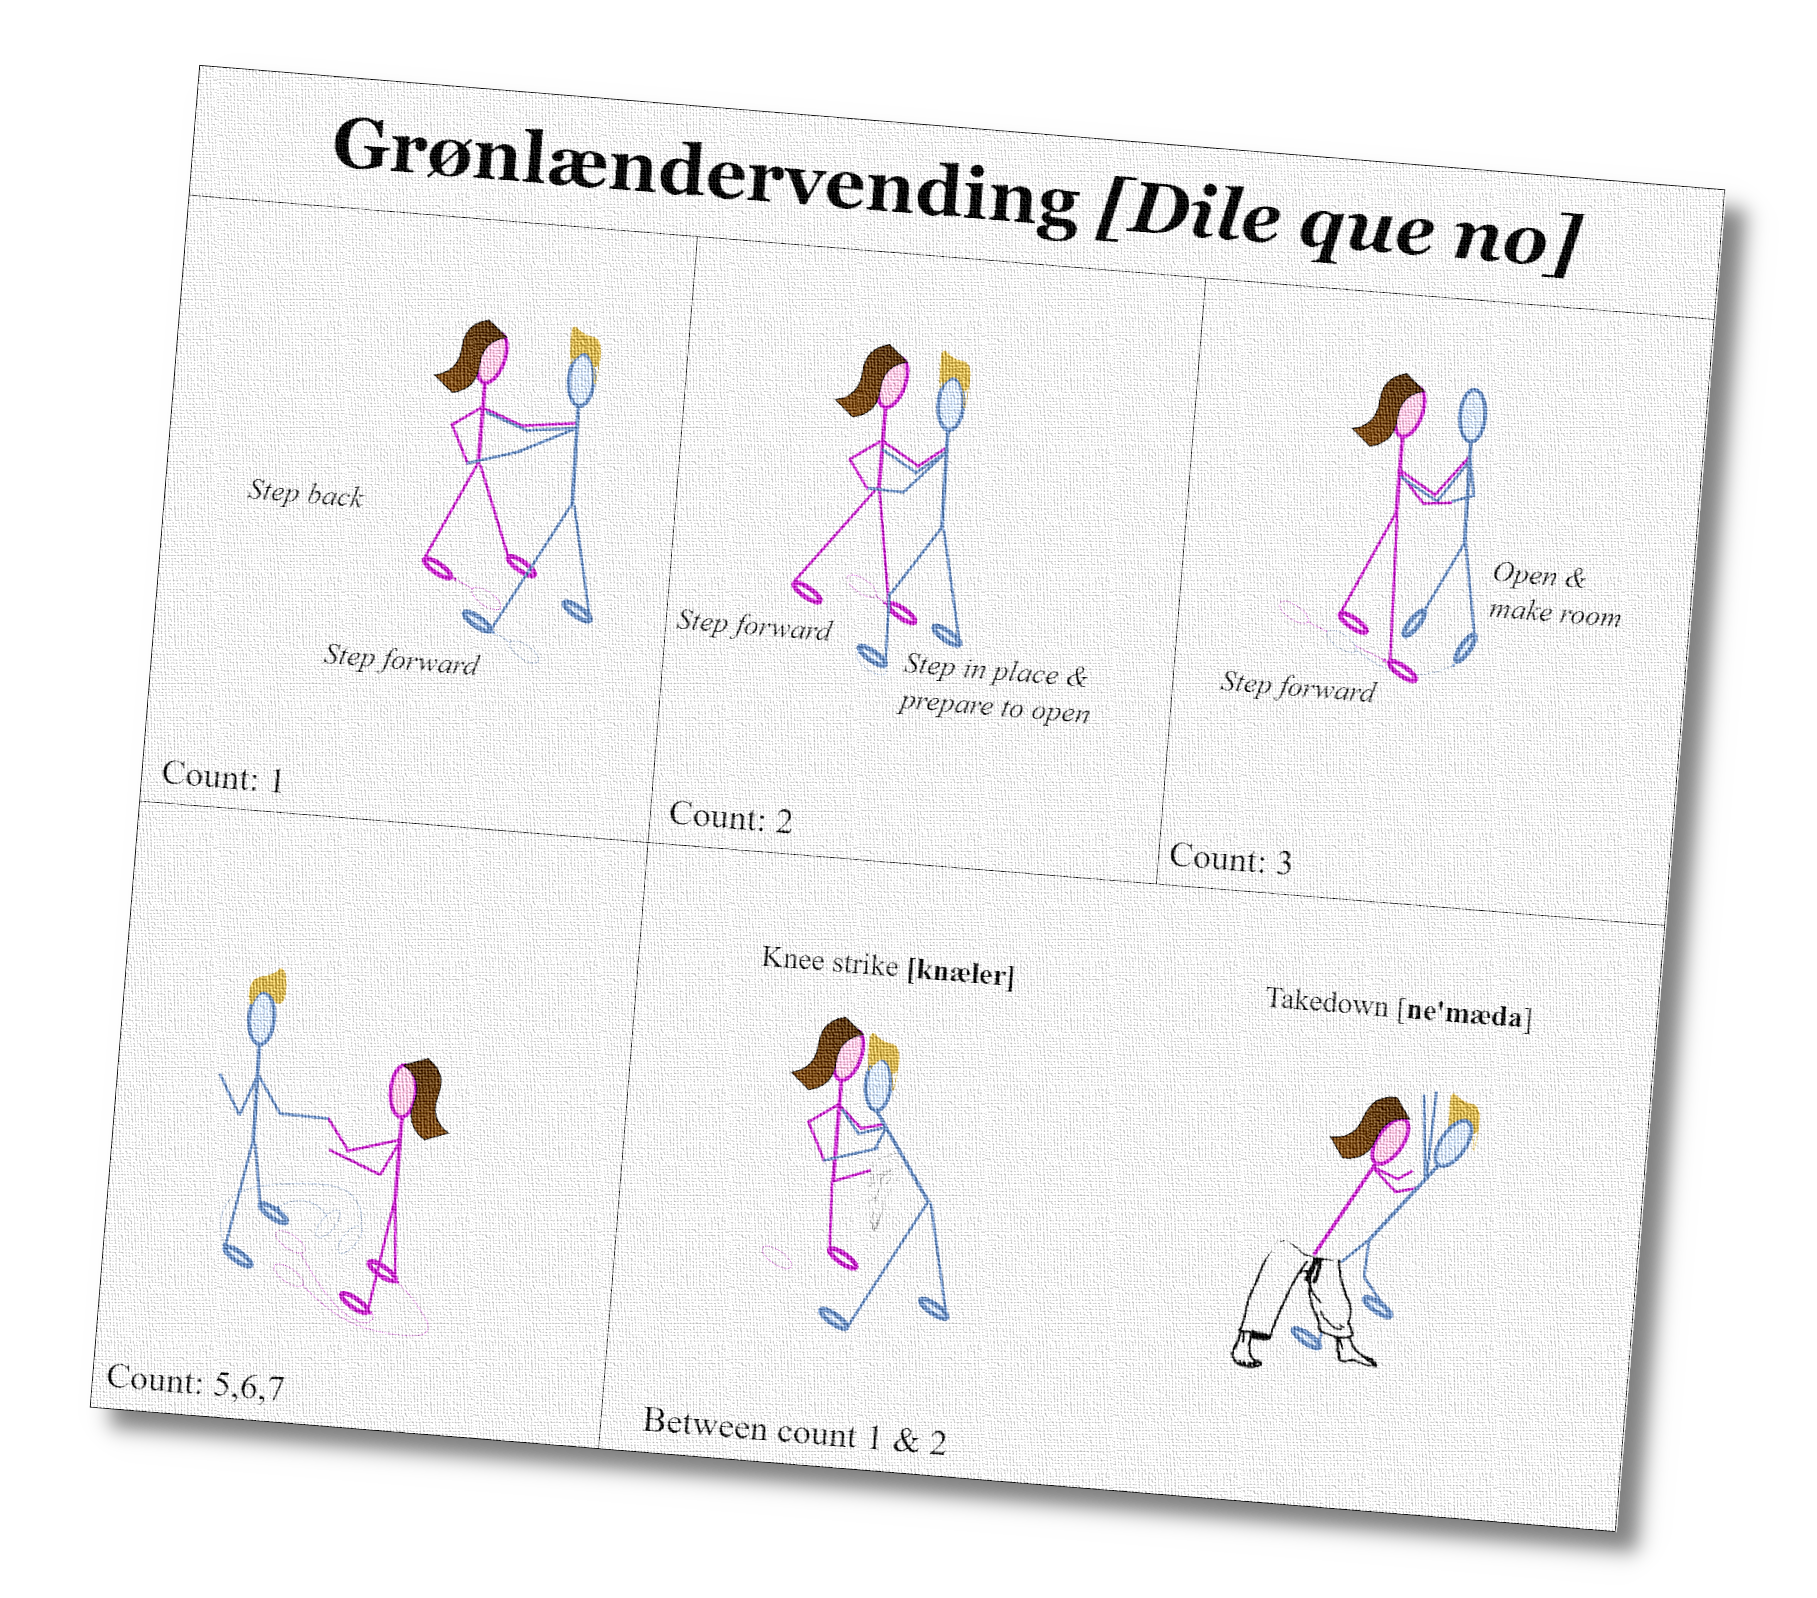
\includegraphics[scale=0.15]{02-Description/diagram-dile-que-no-present}
\end{center}
\subparagraph*{Description}
\Salsadile is in Cuban Salsa used extensively as a part in many other figures, often as the finishing move that brings the two parties back to their starting position, as they change place and direction through the 8 counts. \\
The move is initiated by \dude as he steps towards \gal with his \textbf{left} foot on count 1 and she takes a step back on her \textbf{right} foot. If \dude considers himself a proper gentleman, he will let \gal know what is coming by applying a little more push forward than usual with his left hand. On count 2, \dude takes a small step in-place with his right foot, and prepares to pivot his body leftwards around the axis of his right foot, and \gal takes a small step forward with her left foot. On count 3, \dude completes his pivot and thereby opens an alley for \gal to walk in, as she steps forward with her right foot. \\
Count 5,6 and 7 is pretty much all about the two coming into alignment with each other, both of them now facing the opposite direction of what they did at the start of the move. 
\subparagraph*{Suggestions for attacking}
The  aggresive consumption of territory on count 1 by \dude , opens for some interesting ways for \gal to establish boundaries. If \dude is showing improper balance and is leaning too much forward as he approaches, it is a perfect time for a little impact-testing of his ribcage or abdomen with a powerful \attkneeler (knee strike). Staying in the clinch/BDSM parts of the martial arts, she also has a perfect opportunity to land either a \attrambuk (horizontal elbow strike) or a \attsuperman (diagonally downward cutting elbow), and if on the other hand she really wants to show her interest in him (or she is just more of a \textit{ground n' pound}-style fighter), she could go for the \atttakedown and finish off in mount. 

\pagebreak{}
\section*{\Sovsvuelta [\Salsavuelta]}
\begin{center}
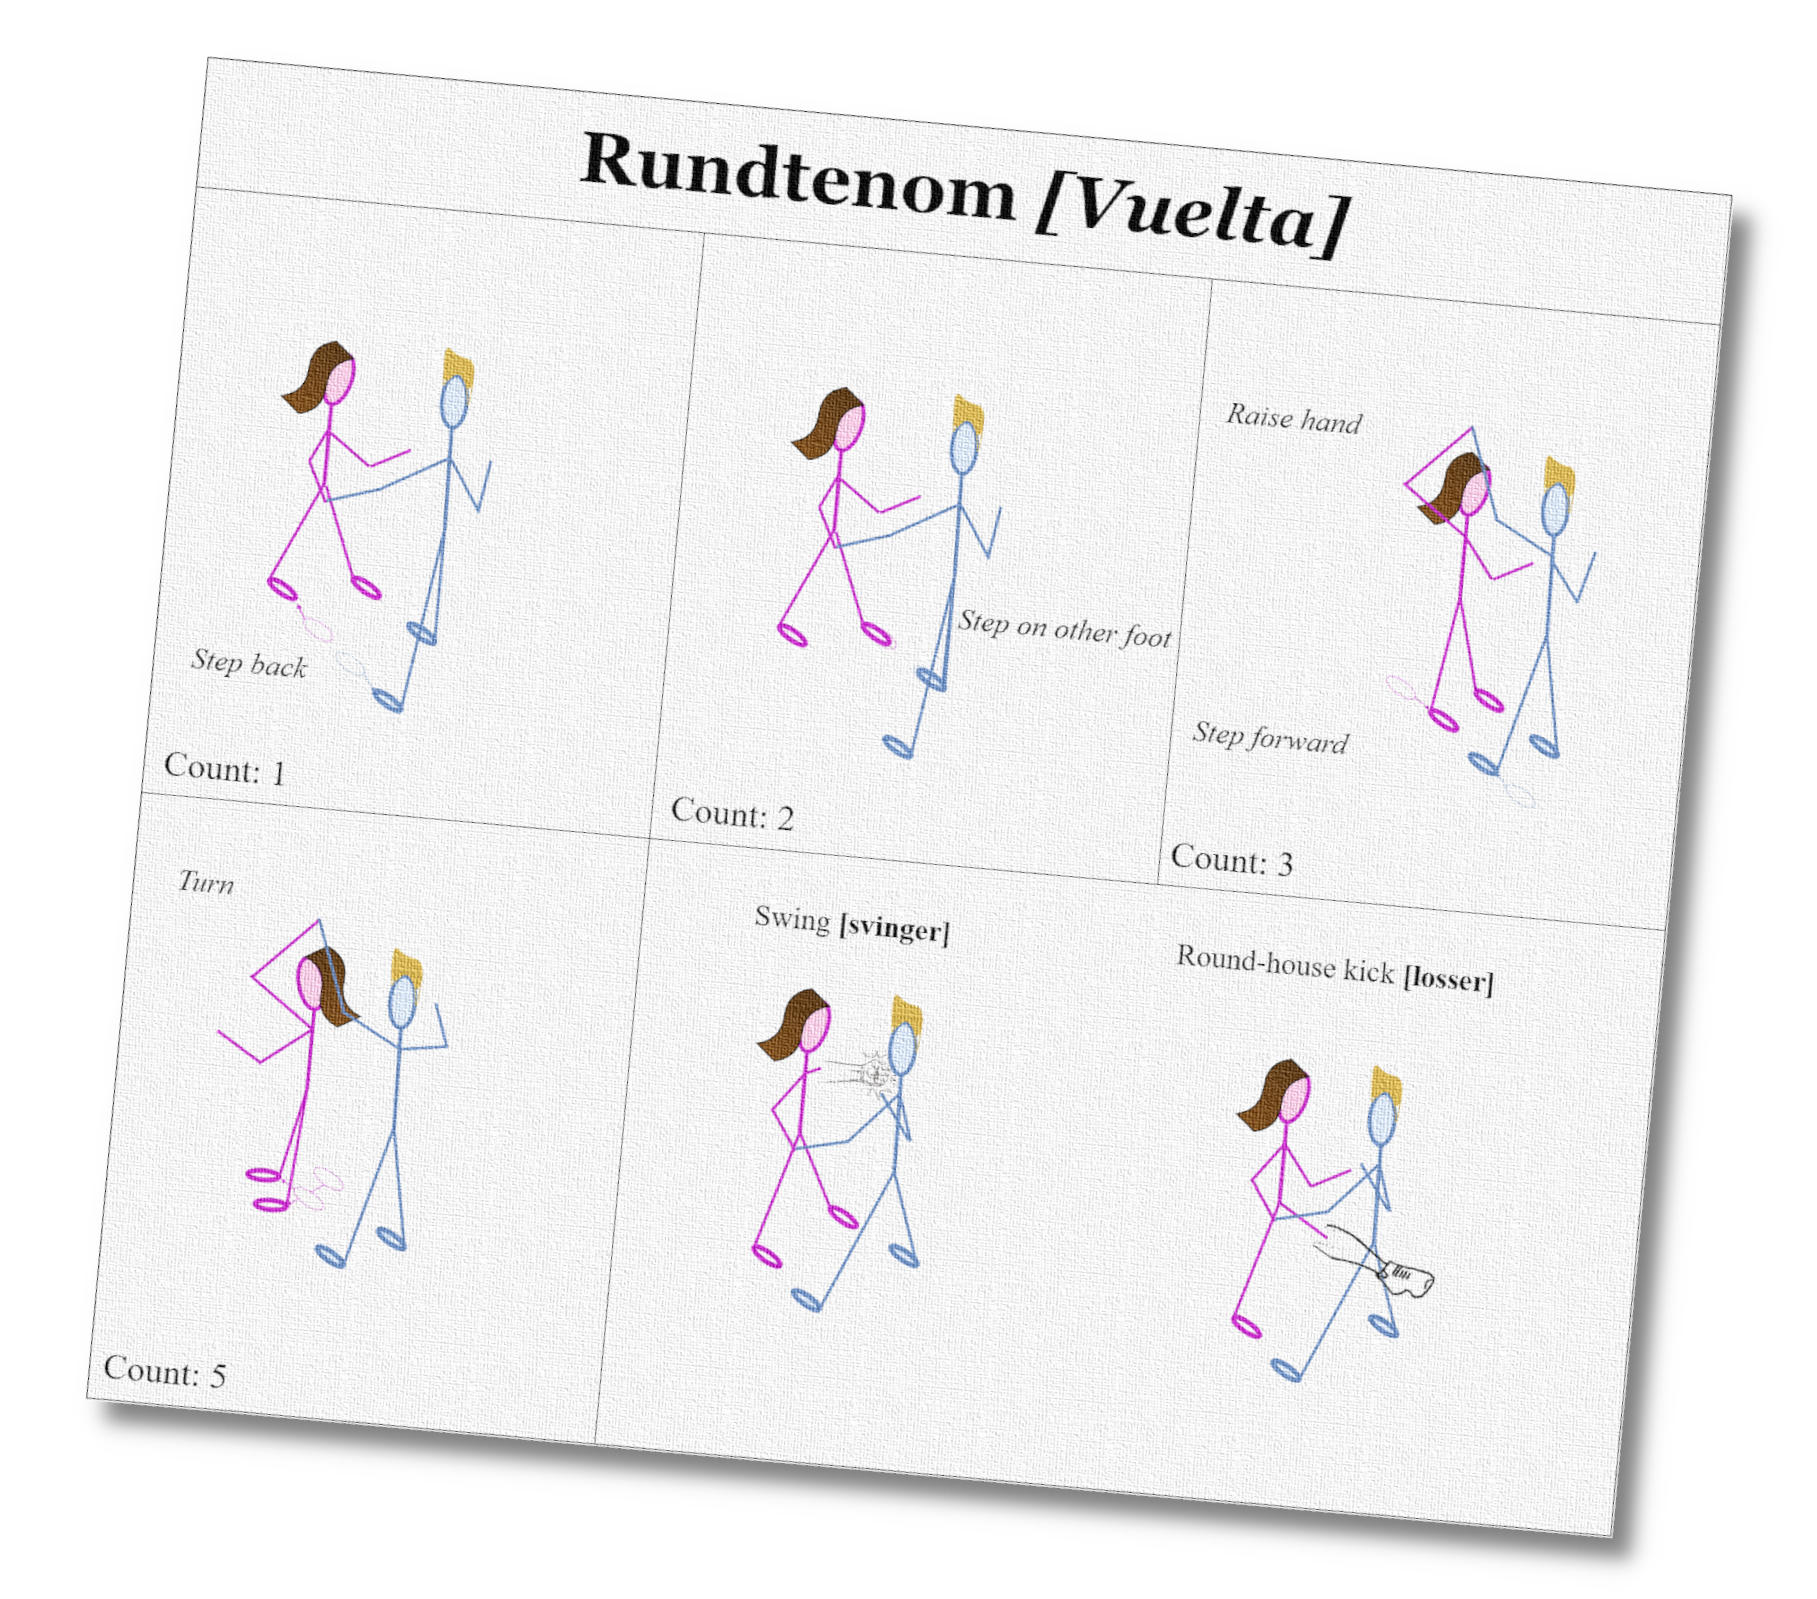
\includegraphics[scale=0.15]{02-Description/diagram-vuelta-present}
\end{center}
\subparagraph*{Description}
As both the Cuban Salsa and the \sovs name for this figure suggests, this move is all about spinning. For \gal at least.\\
The move starts out as \sovsguapea, with both parties stepping back on the $1^{st}$ count, and stepping back to the starting position on the $3^{rd}$ count, but in the \sovsvuelta \dude will raise his left hand on the $3^{rd}$ count to let \gal know that she is about to do some spinning. On count 5, \gal will step forward with her \textbf{left} foot, and proceed to do an outside turn (around her right shoulder)  on counts 6 and 7. 
\subparagraph*{Suggestions for attacking}
Given that the move finishes off with a spinning motion on the part of \gal, any type of attack that can utilize the energy of the spinning motion to generate force will work really well, like for instance:

\begin{itemize}
  \item \attsvinger 
  \item \attack{lav svinger} 
  \item \attlosser
  \item \atthestehilsen
\end{itemize}

\pagebreak{}
\section*{\Sovsenchufla [\Salsaenchufla]}
\begin{center}
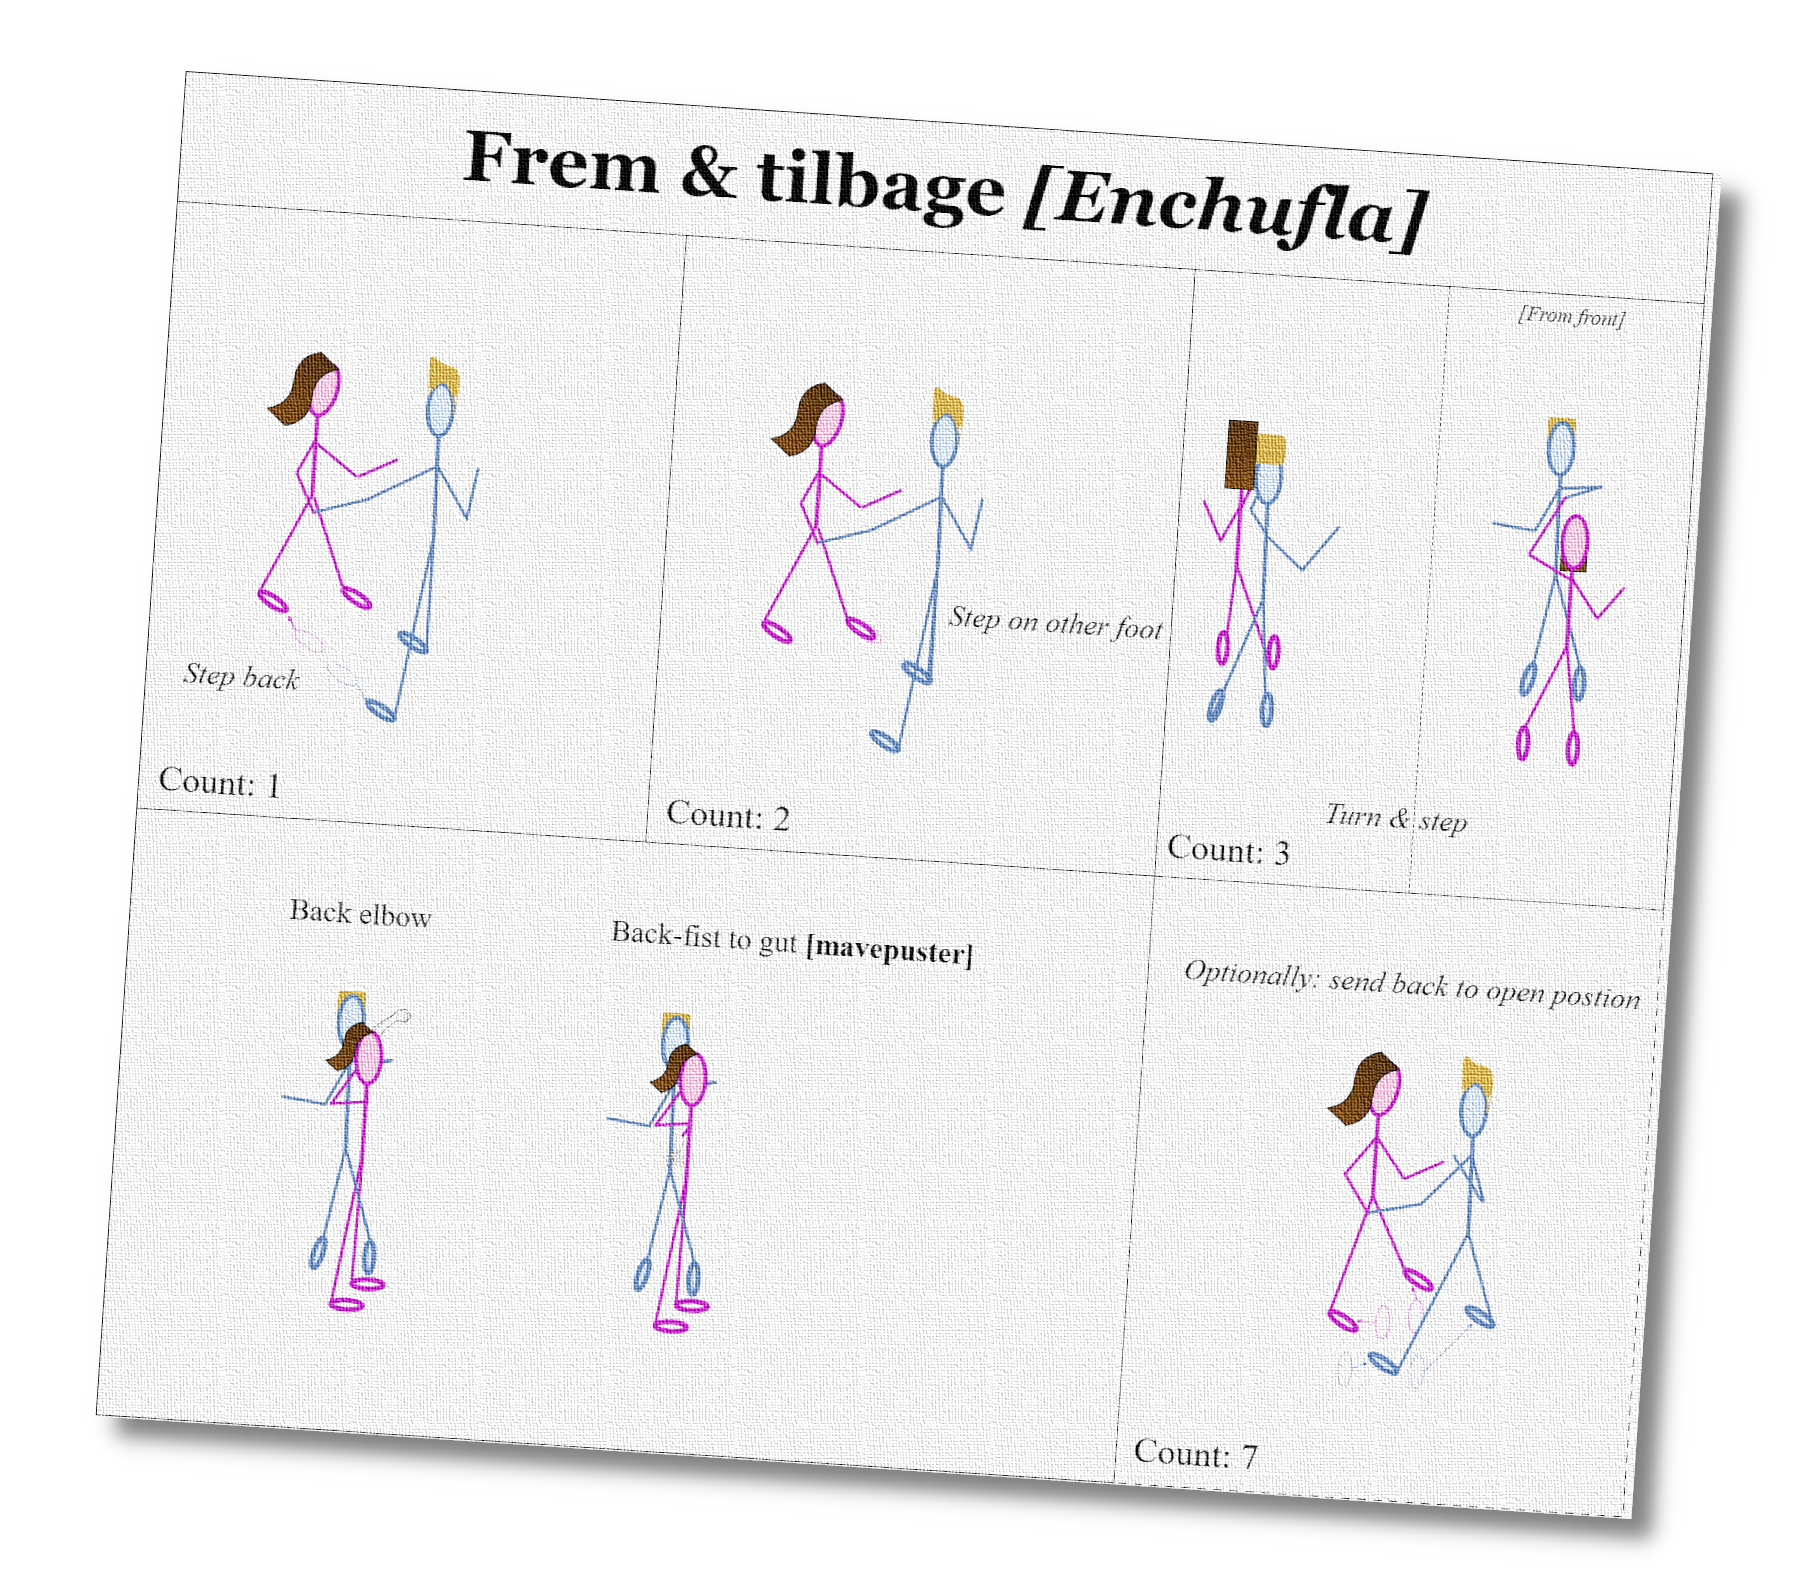
\includegraphics[scale=0.15]{02-Description/diagram-enchufla-present}
\end{center}

\subparagraph*{Description}
\Sovsenchufla is another move for \dude and \gal to exchange places during 8 counts, and is often used in Cuban Salsa as part of other figures. On the $1^{st}$ count, both \dude and \gal will step back as in \sovsguapea, but unlike in \sovsguapea, they will both travel forwards on the $2^{nd}$ and $3^{rd}$ counts. Additionally, on the $2^{nd}$ count, \dude will bring his \textbf{left} hand (which is holding on to \gal's \textbf{right} hand throughout the move) up and infront of their centers, inviting \gal to cross infront of him, with her back to him. At the end of the $3^{rd}$ count, both parties turn towards each other. Counts 5, 6 and 7 proceed as for \sovsguapea. 
\subparagraph*{Suggestions for attacking}
This is one of those moves that really allows \gal to rid herself of a drunken or unattentive partner! If she starts her spinning motion as she crosses infront of \dude, and hits him with a \attkaffekage (back elbow) (thereby completing the Danish saying: \textit{``Kaffe \& kage, frem \& tilbage''} to the face, she will send an unambigous message to \dude, that he should look for another place to spend the night. Of course, it may be the case that \dude is not as drunk/unattentive as he looks, and is able to catch the elbow in-flight, and in this case, he has little choice but to push her back in what is known in \sovs as \sovsenchufla$^{2}$ [\figsalsa{enchufla doble}]. \\
\gal also has the option to postpone her spinning motion and attack until the $3^{rd}$ count, but will likely have to throw an attack with a longer reach at \dude, like for instance a \attbagknytter or \attsideaxe.


\pagebreak{}
\section*{\Sovsvacilala [\Salsavacilala]}
\begin{center}
\includegraphics[scale=0.15]{02-Description/diagram-vacílala-present}
\end{center}
\subparagraph*{Description }
\Sovsvacilala is initiated already on the preceeding move (typically \sovsguapea), as \dude let's \gal know that \textit{``something is up'}', by pushing a little harder than usual with his free hand in order to open up their position. As such, \sovsvacilala starts with the both of them looking in the same direction.
On the first count, \dude gently motions \gal's right hand in a spinning motion inwards as he steps to move past her on the outside. \gal performs a single (or double/tripple) spin moving past and away from \dude. 
On the 5-count \dude steps toward \gal, in order to close the distance and prepare for \sovsdile.

\subparagraph*{Suggestions for attacking}
Given the rather large distance between the 2 on count 4 and 5, and the fact that \gal is free from contact with \dude and hence enjoys full freedom of motion, it is a great time for her to show off her athletic abilities and hit him with some long-distance kicking. \gal can opt for a \atttrykker directed towards \dude's torso, or she could adjust her body sideways and go for a \attsidetrykker. She can go for the power-up and preface the \attsidetrykker with stepping into the kick with her rear leg, which is sure to send \dude flying if he is not attentive which will most certainly aid \gal in establishing dominance on the dance floor.\\
If \gal feels like showing off, she can pull out the old kick-combo classic, the \attfootjuglar faking a round-house kick and following up with a \atthestehilsen from the opposite foot.  

\chapter*{The \sectionsovs nomenclature}
Names are actually pretty useful, maybe even moreso than you usually think. Take it from someone who takes an extremely long time memorizing the names of new acquaintances: not being able to properly address someone/something and having to resort to ``Hey you!'' and ``That thing over there!'' get's old pretty fast. This same principle of course also applies to \sovs: it's a lot more tiresome to say: ``he did that that move where he raised his hand and she turned and swung a fist at him'' than ``he took her for a \textit{rundtenom} and she responded with a \textit{svinger}''. \\
More than just allowing for precise communication of the actions on the dance floor, the nomenclature of \sovs also captures an essential part of Danish culture and it's love for naming things in a kind of naughty and street-wise manner, known and cherised from classics such as: \textit{bingo-lingo} and \textit{pølse-slang}.

\section*{Names of figures}
As any valid figure from Cuban Salsa is also a valid figure in \sovs, the names of figures are more or less direct translations of figures from Cuban Salsa.


\begin{center}
\begin{tabularx}{1\textwidth}{
  |
      >{\raggedright\arraybackslash}X  
      >{\raggedright\arraybackslash}X  
  |
}
\hline
\figsalsa{Name in Cuban Salsa} & \figsovs{Name in \sovs} \\
\hline
\Salsaguapea & \Sovsguapea\\
\Salsavuelta & \Sovsvuelta  \\
\Salsavamos & \Sovsvamos \\
\Salsadile & \Sovsdile \\
\Salsaenchufla & \Sovsenchufla \\
\Salsavacilala & \Sovsvacilala \\
\hline
\Salsauno & \Sovsuno  \\
\Salsados & \Sovsdos \\
\Salsasetanta & \Sovssetanta \\
\Salsasetantayuno & \Sovssetantayuno \\
\Salsasetantaydos & \Sovssetantaydos \\
\hline
\end{tabularx}
\end{center}


\section*{Names of attacks}

\begin{tabularx}{1\textwidth}{
  |  >{\raggedright\arraybackslash}X 
      >{\raggedright\arraybackslash}X  
  |
}
\hline
\attackdesc{What} & \attack{Name in \sovs} \\
\hline
\attackdesc{Straight punch} & \Attknytter \\
\attackdesc{Swing/hook} & \Attsvinger \\
\attackdesc{Fake punch, punch to stomach} & \Attflemming \\
\attackdesc{Backfist} & \Attbagknytter \\

\attackdesc{Sideways knife-hand}  & \Attsideaxe \\

\attackdesc{Round-house kick} & \Attlosser \\
\attackdesc{Front/push kick} & \Atttrykker \\
\attackdesc{Side kick} & \Attsidetrykker \\
\attackdesc{Back kick} & \Atthestehilsen \\
\attackdesc{Fake round-house to Heste-hilsen} & \Attfootjuglar \\

\attackdesc{Horizontal elbow} & \Attrambuk\\
\attackdesc{Diagonally downward slicing elbow} & \Attsuperman\\
\attackdesc{Back elbow} & \Attkaffekage \\
\attackdesc{Knee strike} & \Attkneeler \\

\attackdesc{Take down} & \Atttakedown \\
\hline
\end{tabularx}





\chapterize{Tilsmagning}
  {
   Når sovsen har opnået den ønskede konsistens, smages den til med krydderier og andre smagsstoffer, indtil den ønskede smag er opnået. \\

  \chapgap

  Skal sovsen bruges til flæskesteg, anbefales det at tilsætte gode mængder svinefedt og ribsgele.\\

  \chapgap

  Skal sovsen bruges som ostesovs til lasagne, anbefales gode mængder mozzarella-ost og en smule muskat-nød. Glem ikke salt \& peber.
  }
  {
When the sauce has achieved the desired consistency, it is flavored with spices and other flavorings until the desired flavor is achieved.\\

  \chapgap

  If the sauce is to be used for roast pork, it is recommended to add good amounts of lard and redcurrant jelly.\\ 

  \chapgap

  If the sauce is to be used for lasagne, good amounts of mozzarella cheese and a little nutmeg are recommended. Don't forget salt \& pepper.  
}{03-Outro/chapter-deco}

\chapter*{Your \sectionsovs drip}
\textit{``Does \sovs have a uniform?''} \textit{``Do you think she'll go for this \textit{dobok}/\textit{dashiki}/\textit{toque} combo?''} \footnote{Sure... You're good!} \textit{``Do you think the females will digg this forrest green and sunflower yellow track suit/skull cap mix?''} \footnote{I don't know man... sounds a little sketchy. Maybe. Try not to be fat}\\
Unfortunately, hitting the dance floor isn't as simple as just rolling out of bed and going to the club in your jammies, but will involve such boring practicalities as picking out clothes to wear that won't have the doormen ``randomly'' picking you out at the entrance and preemptively beating your silly-looking ass with a nightstick. Good news is though, that in terms of \sovs, there are is no fashion police: you do you!\\
However, seeing as the music at most dancing venues is rather loud and your cauliflowered ears may not function the way they used to, you may want to find a non-verbal way to let your dance partner know that you are a \sovseneer \footnote{especially if you are a \dude in a country that enforces some kind of legislation against unprovoked acts of violence, letting \gal know that she is not liable to criminal charges if she punches you in the face, is hella \textbf{gentleman}}  and besides from tattooing \sovs on your extremeties, expressing it through your choice of clothing seems like the obvious idea. Now, I am no fashion guru. I would even go so far as to say, that given predicate $p$ such that $p(a,b)$ is \textit{true} for persons $a$ and $b$ \textit{iff.} $a$ knows more about fashion than $b$, it holds that 

\begin{equation*}
P(p(a_x, \pmb{Sunetiago} \; \pmb{Hansen}) \; is \; \pmb{true})) \geq 96.45\%, \; \forall \; a_x  \in  S_{10} 
\end{equation*}

where $S_{10}$ is the set consisting of human beings older than $10$ years of age.\\
Nonetheless, in the following I will provide some suggestions for inspiration to your \sovs-uniform. Whether the bouncers at the club will let you in and/or if they will get you beat up on the way to/from the club, I have no idea. The suggestions should mostly apply to both \dude and \gal, but please apply common sense. 

\newpage
\subsection*{Lower body}
Most clothing made for martial arts, is made with durability and flexibility in mind, so I suggest looking towards the martial arts for inspiration when it comes to finding appropriate \sovs leg-wear. You could repurpose the pants from your old \textit{Taekwondo} or \textit{Kong Fu} uniform, or if you feel like showing off your new tats and sturdy legs, you could go for the familiar \textit{Muay Thai} shorts. 

\vspace{10pt}

\begin{center}
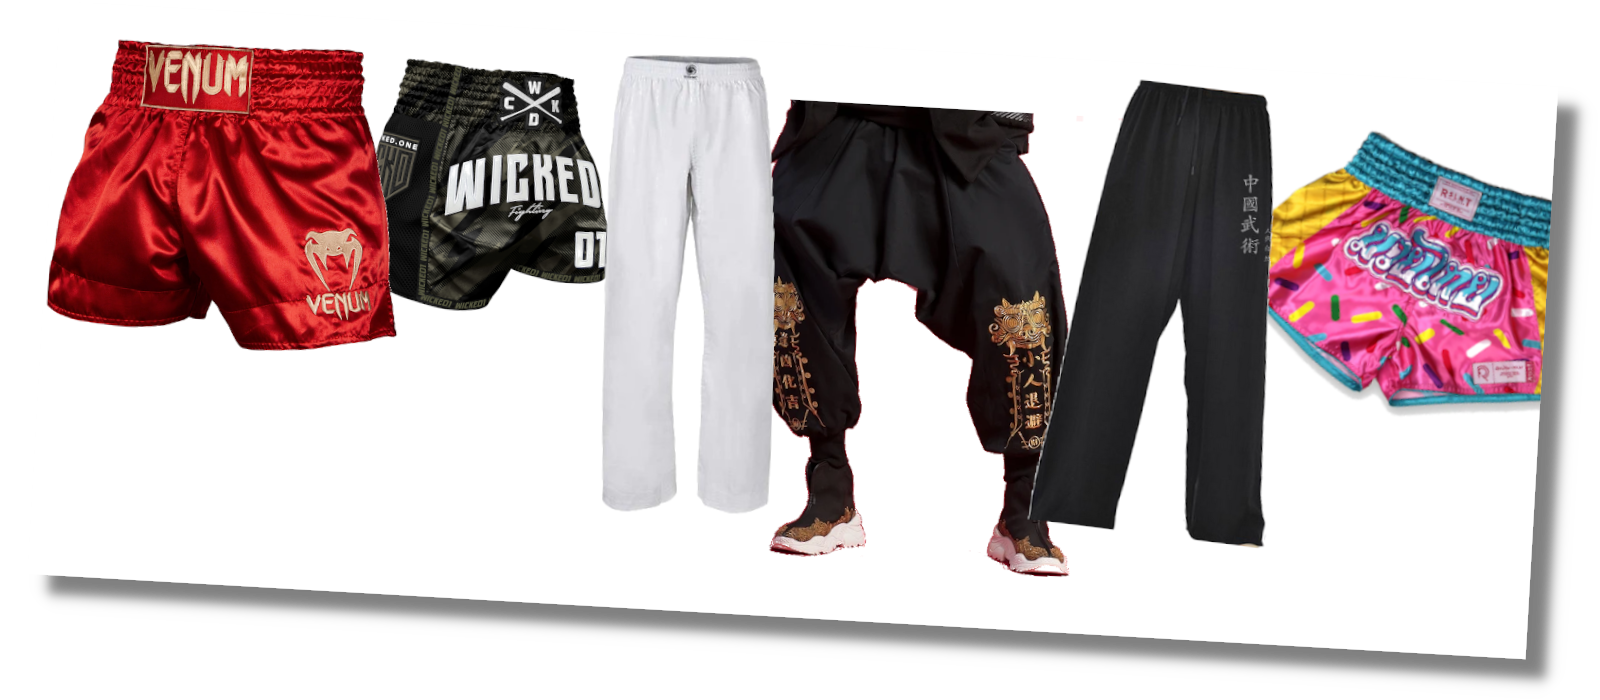
\includegraphics[scale=0.3]{03-Outro/lower-body-final}
\end{center}


\newpage
\subsection*{Upper body}
Do you remember the last time you went to a party in a shazzy Hawaii-shirt, and everyone was like: \textit{``OMG, that shirt is HORRIBLE!''}. No? That's because it has never happened, and that's because Hawaii shirts at dance parties are an evergreen. In general, I recommend looking towards the equator when picking out upper body wear for \sovsing. 

\vspace{10pt}

\begin{center}
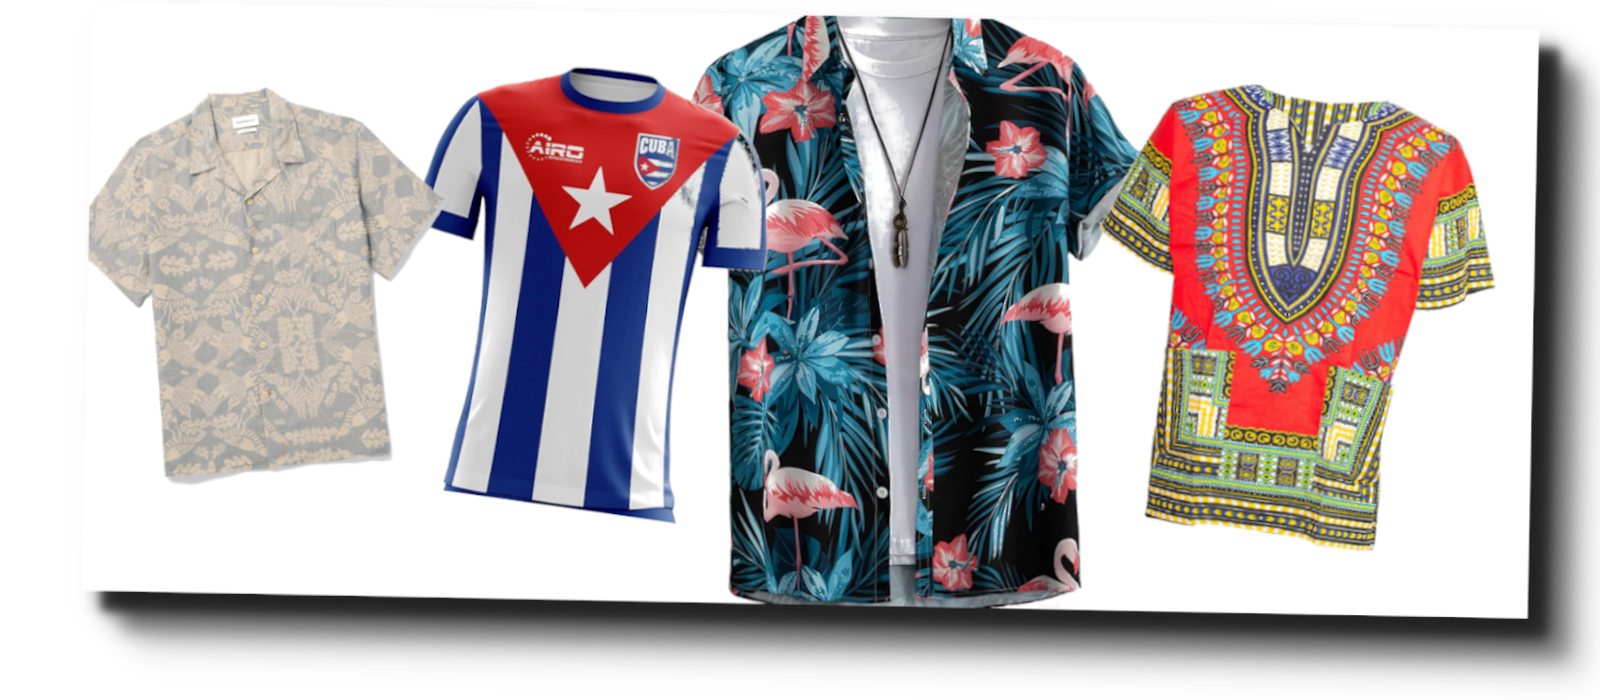
\includegraphics[scale=0.3]{03-Outro/upper-body-wear-final}
\end{center}

\vspace{10pt}

\newpage
\subsection*{Accessories}
I once, while driving a car, tuned into a radio program starring 2 metrosexuals talking about really expensive watches. I don't remember much from that show, but they seemed to make a great deal about \textit{accessorizing} your wardrobe. Personally, the only accessory I have ever  bought has been cufflinks \footnote{a friend of mine gifted me some expensive work-shirts he had become too fat to use himself, and for a while I was wondering what type of \textbf{\textit{absolute scoundrel}} gives away shirts without those sleeve buttons}, but I can totally see how there are some really cool ways to turn your regular clubbing wardrobe into genuine \sovs gear with just a couple of accessories.

\begin{center}
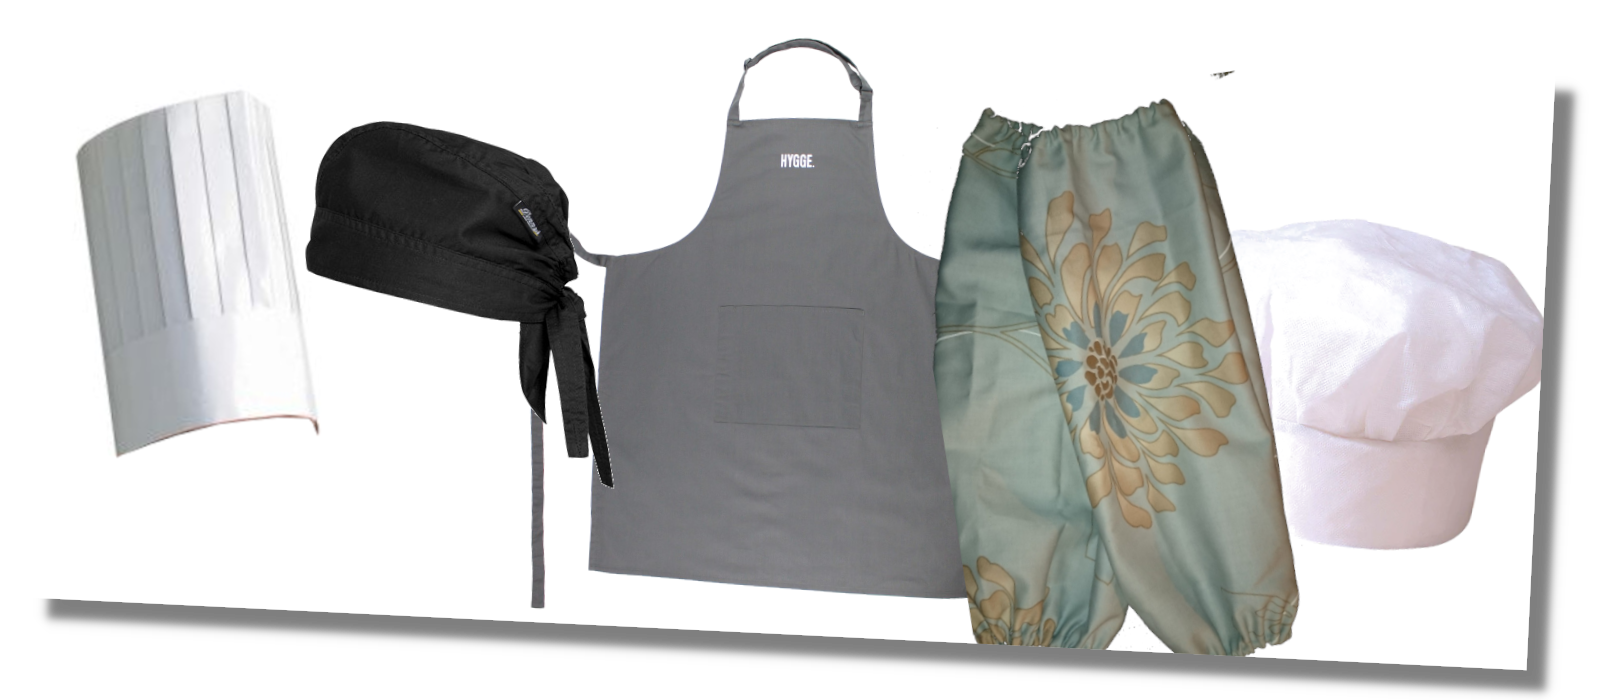
\includegraphics[scale=0.3]{03-Outro/accessories-final}
\end{center}


\end{document}